\newcommand{\reqs}{Systemkrav}
\newcommand{\slutbrugere}{Slutbrugere}
\newcommand{\funcreqs}{Funktionelle}
\newcommand{\nonfuncreqs}{Ikke-Funktionelle}
%\newcommand{\nonfuncreqs}{Kvalitetskrav}


\section{\reqs}
\begin{frame}{\reqs}
	\begin{itemize}
		\item System baseret p� krav
		\item<2-> Krav kommer fra slutbrugere
	\end{itemize}
\end{frame}



\begin{frame}{\reqs}{\slutbrugere}
	\begin{itemize}
		\item Kategorier
		\begin{itemize}
			\item Brugere af projekt grupper
			\item Managere af projekt grupper
		\end{itemize}
		\item Dimensioner
		\begin{itemize}
			\item Type
			\item Fakultet
			\item Institut
			\item LMS erfaring
		\end{itemize}
	\end{itemize}
\end{frame}

\begin{frame}{\reqs}{\slutbrugere}
	\begin{figure}
		\centering
			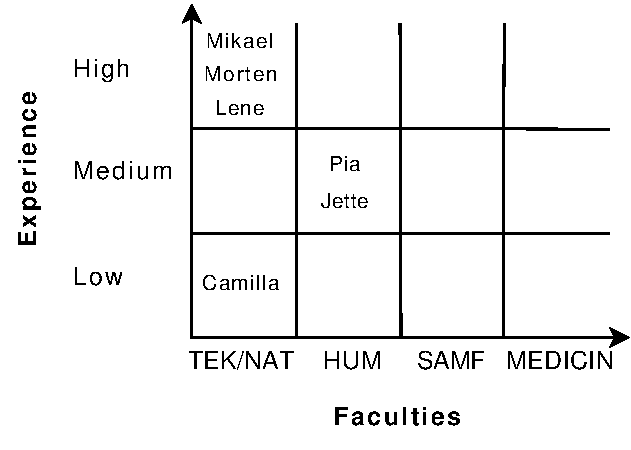
\includegraphics[width=\textwidth]{../report/images/administratorsOfPG.pdf}
		\label{fig:administratorsOfPG}
	\end{figure}
\end{frame}

\begin{frame}{\reqs}{\slutbrugere}
	\begin{figure}
		\centering
			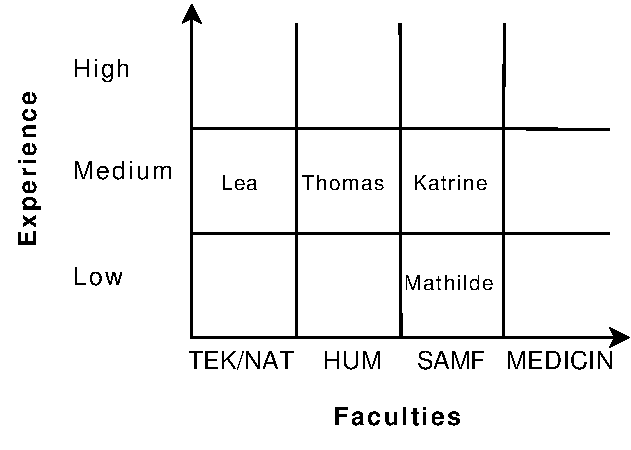
\includegraphics[width=\textwidth]{../report/images/MembersofpROJECTgROUJP.pdf}
		\label{fig:MembersofpROJECTgROUJP}
	\end{figure}
\end{frame}

\begin{frame}{\reqs}{\funcreqs}
	
\end{frame}








